\documentclass[12pt]{article}
\usepackage{indentfirst}
\usepackage{url}
\usepackage{pgf-pie}
\usepackage{graphicx}
\usepackage{enumitem}
\usepackage{tikz}
\usepackage{amsmath}

\newlength{\itemimagewidth}
\setlength{\itemimagewidth}{1.5cm}

\newlist{roadmap}{enumerate}{1}
\setlist[roadmap]{label={},leftmargin=*}

\newcommand{\roadmapitem}[3]{
  \item \begin{tikzpicture}[baseline={(0,-0.5)}]
    \node[anchor=west,inner sep=0pt,outer sep=0pt,minimum height=2em,minimum width=\itemimagewidth] (image) at (0,0) {\includegraphics[width=\itemimagewidth]{#1}};
    \node[anchor=west,inner xsep=5pt] at (image.east) {\parbox[t]{\dimexpr\linewidth-\itemimagewidth-5pt}{\textbf{#2}\par #3}};
  \end{tikzpicture}
}

\setlength{\oddsidemargin}{27mm}
\setlength{\evensidemargin}{27mm}
\setlength{\hoffset}{-1in}

\setlength{\topmargin}{27mm}
\setlength{\voffset}{-1in}
\setlength{\headheight}{0pt}
\setlength{\headsep}{0pt}

\setlength{\textheight}{235mm}
\setlength{\textwidth}{155mm}

\pagestyle{plain}

\renewcommand{\thefootnote}{\fnsymbol{footnote}}
\renewcommand{\labelitemi}{$\bullet$}

\begin{document}
\baselineskip 11pt


\begin{center}
  \textbf{\Large Swaptor Whitepaper} \\

  \vspace{1.5cc}
  { \sc Marko Ivanković$^{1}$}\\

  \vspace{0.3 cm}

  {\small $^{1}$Berry Block, marko@berryblock.io}
\end{center}
\vspace{1.5cc}

\begin{abstract}
  \noindent  Peer-to-peer (P2P) swaps on blockchain have the potential to greatly benefit users by eliminating the need for intermediaries in the exchange of assets. However, the use of P2P swaps on blockchain also presents several challenges, including trust issues that must be addressed in order to ensure their success.  Since there is no intermediary to oversee the exchange of assets, users must rely on the trustworthiness of the other party to the transaction. In the absence of a trusted third party, it is difficult to verify the authenticity and quality of the assets being exchanged, which can lead to disputes and losses for users.
  \\ \indent Furthermore, P2P swaps on blockchain are subject to potential security risks, such as hacking and fraud. Since the transactions are conducted directly between users, there is a greater risk of malicious actors attempting to exploit vulnerabilities in the system. This risk is exacerbated by the fact that blockchain transactions are irreversible, meaning that users have no recourse if their assets are stolen or lost.
  \\ \indent In this paper we describe Swaptor, a decentralized P2P exchange dapp which aims to eliminate problems mentioned above.

  \vspace{0.95cc}
\end{abstract}

\newpage

\tableofcontents

\newpage

\section{Architectural Overview} \label{form}
\indent As most modern dapps, Swaptor's architecture is a mix of on-chain and off-chain components:
\begin{itemize}
  \item \textbf{On-chain}: Smart contracts
  \item \textbf{Off-chain}: Backend, Frontend and Database
\end{itemize}

\subsection{On-chain Architecture}

\indent Smart contracts are written in Solidity, and their architecture is designed to be minimalistic.
Specifically, the Swaptor contract is a singular entity whose sole purpose is to verify digital signatures
and execute swaps upon successful verification. Digital signatures encode the specific terms under which a given swap is considered valid.

\subsubsection{Signatures}

In order to verify the signature, the smart contract must possess both the original swap elements
and the signature itself. Prior to being passed as an argument to one of the \textit{acceptSwap} functions,
these elements are encoded using the \textit{abi.encode} function. The signature is generated by creating a
\textit{keccak256} hash of the encoded arguments and signing it with the private key belonging to the seller.
This method dramatically reduces the gas fees because the seller never had to transfer their assets to Swaptor contract.

\subsubsection{Swap types}

At present, Swaptor facilitates the swapping of ERC-721 and ERC-20 tokens, enabling the execution of any combination of swaps involving these types of tokens.
In the future, Swaptor intends to extend its support to include native currency and ERC-1155 tokens.

\subsubsection{Fees}
To accept the swap, an address will need to pay a fixed fee of \$$5$ in the native currency, which is calculated using Chainlink oracles\cite{chainlink}. It should be noted that the fee is not fixed and may be subject to change.

  \subsection{Off-chain Architecture}

  \subsubsection{Backend}
  The purpose of the backend is to reduce the number of operations on the blockchain,
  which would result in higher gas fees paid by users. It also caches some information
  retrieved from the blockchain to improve the user experience, such as reducing wait
  times. Upon client request, it retrieves details about swaps, including the original
  swap terms and signature.

  \subsubsection{Frontend}
  The Swaptor frontend application is a user interface that allows users to interact
  with the Swaptor protocol on the supported networks. It enables users to easily swap
  supported token types without the need for a centralized exchange. Each user is capable
  of creating, deleting, sharing and accepting a swap. The application is accessible through a
  web browser or mobile device and is designed to be user-friendly and intuitive.

  \section{Tokenomics}

  \subsection{Token Mechanics}

  The price of Swaptor Token (SWPTR) is influenced by several factors,
  including activity on the Swaptor Protocol, the price of Ether,
  and liquidity pool activity. As mentioned earlier, every time a
  successful swap occurs, a fixed fee in the native currency is
  exchanged for SWPTR token in the Ether/SWPTR liquidity pool.
  The amount of SWPTR token is then burned, leading to an increase
  in the price of SWPTR token.

  Given that Ether is on the other side of the pool, the price of
  SWPTR is directly affected by the price of Ether. The decision to
  use Ether as the currency for the exchange fee is based on the fact
  that users already pay gas fees in Ether, and adding an additional
  swap would result in gas wastage. Moreover, Ether is the backbone of
  many other coins, and a decrease in its price would effectively
  eliminate a significant portion of the Ethereum DeFi ecosystem.




  \subsection{Token Allocation}

  Total of $1000000$ (one million) SWPTR tokens will be minted and distributed over time as described by Figure \ref{fig:pie-chart}.

  \begin{figure}[h]
    \centering
    \begin{tikzpicture}
      \pie{20/Public sale, 30/VC, 16/Team, 18/Community, 16/Liquidity pool}
    \end{tikzpicture}
    \caption{Pie chart showing the distribution of tokens}
    \label{fig:pie-chart}
  \end{figure}

  The tokens allocated to the community, as illustrated in Figure \ref{fig:pie-chart}, will be distributed from the Swaptor contract.
  Tokens that are not distributed to venture capitalists will be available for purchase by the public. Any unsold tokens from the public sale will be allocated to the team.
  Upon swap execution, both the buyer and seller will be granted a single SWPTR token.
  Buyer and seller are motivated to hold the token as its price will grow proportional to Swaptor activity.

  \newpage

  \subsection{Utility}
  At present, the SWPTR token serves only to reflect the strength of the
  project and the level of traction it has gained. Rational investors
  who believe in the project's bright future may choose to hold the
  token, as its price increases every time a swap is executed.

  During the community token distribution phase, it is expected that
  the price increase will be slightly lower, as two SWPTR tokens will
  be released from the Swaptor contract, giving actors the option to swap
  them for Ether. However, this scenario is highly unlikely, as the
  amount earned during this phase will be negligible, partly due to
  the gas fees required for swapping. Any impact on the price of SWPTR during
  community distribution phase due to actors who decide to swap tokens
  for Ether is partially dampened by the swap and burn mechanism executed
  by the Swaptor contract.

  \subsection{Vesting}
  All tokens will be released within a 750 day (2 years and 20 days) period.
  Token vesting is described by the following calculation:
  \begin{equation}
    T_{ps} = 0.34 \cdot T_{s} = 340000
  \end{equation}

  \begin{equation}
    T_{vc} = 0.22 \cdot T_{s} = 220000
  \end{equation}

  \begin{equation}
    T_{t} = 0.16 \cdot T_{s} = 160000
  \end{equation}

  \begin{equation}
    T_{sum}  = T_{ps} + T_{vc} + T_{t} = 720000
  \end{equation}

  \begin{equation}
    t = 750\;\text{days} = 6.48 \times 10^7\;\text{s}
  \end{equation}

  where $t$ denotes the total vesting period \\

  \begin{equation}
    G    = \frac{T_{sum}}{t} = 960\;\text{tokens/day}
  \end{equation}

  where $G$ denotes the amount of tokens released on a daily basis \\



This vesting will apply to tokens acquired by venture capitalists,
public sales, and the team. This measure has been introduced to
increase the trust of the community by regulating token dumping and
aligning the interests of the team with the project itself.

\newpage

\section{Roadmap}

\begin{roadmap}
  \roadmapitem{swaptor.png}{Q3 2023}{
    Deployment of Swaptor contracts to Ethereum mainnet.
  }

  \roadmapitem{swaptor.png}{Q4 2023}{
    Public swaps - listed on Swaptor website.
  }

  \roadmapitem{swaptor.png}{Q2 2024}{
    Swaptor messaging \& notification system - enabling direct communication between users through Swaptor website
  }

  \roadmapitem{swaptor.png}{Q3 2024}{
    Support for remaining token standards
  }
\end{roadmap}

\begin{thebibliography}{9}
  \bibitem{chainlink} What is an oracle in blockchain? explained | chainlink, \url{https://chain.link/education/blockchain-oracles}
\end{thebibliography}

\end{document}